\documentclass{classrep}
\usepackage[utf8]{inputenc}
\frenchspacing

\usepackage{graphicx}
\usepackage[usenames,dvipsnames]{color}
\usepackage[hidelinks]{hyperref}
\usepackage{lmodern}
\usepackage{graphicx}
\usepackage{placeins}
\usepackage{url}
\usepackage{amsmath, amssymb, mathtools}
\usepackage{listings}
\usepackage{fancyhdr, lastpage}

\pagestyle{fancyplain}
\fancyhf{}
\renewcommand{\headrulewidth}{0pt}
\cfoot{\thepage\ / \pageref*{LastPage}}

%--------------------------------------------------------------------------------------%
\studycycle{Informatyka stosowana, studia dzienne, II st.}
\coursesemester{I}

\coursename{Wprowadzenie do Data Science i metod uczenia maszynowego}
\courseyear{2020/2021}

\courseteacher{mgr inż. Rafał Woźniak}
\coursegroup{Wtorek, 13:15}

\author{%
    \studentinfo[239671@edu.p.lodz.pl]{Jan Karwowski}{239671}
}

\title{Zadanie 1.: Problem set 1}

\begin{document}

\maketitle
\thispagestyle{fancyplain}

\section{Wprowadzenie}

Pośród wielu różnych błędów i manipulacji, których można dokonać z wykorzystaniem statystyki, dość
częstym jest mylenie (umyślne lub przypadkowe) wartości \emph{względnych i bezwzględnych}.
Najprostszym przykładem tego rodzaju błędu jest przedstawienie na wykresie wartości bezwzględnej
pewnej cechy dla np. danych obszarów lub kategorii, podczas gdy z wartości względnych (z
uwzględnieniem rozmiaru poszczególnych grup) wynika zupełnie co innego. W ten sposób można
zmanipulować społeczeństwo, przykładowo prezentując poparcie wyborców w okręgach wyborczych.

\section{Przykład 1: Wartość bezwzględna zarażeń koronawirusem w województwach}

Rysunek \ref{wzgledne_bezwzgledne} (źródło
https://www.gov.pl/web/koronawirus/wykaz-zarazen\-koronawirusem-sars-cov-2) pokazuje liczbę zarażeń
koronawirusem z pojedynczego dnia, dla poszczególnych województw w Polsce. Jak widać z tego rysunku,
najgorsza sytuacja jest w województwie mazowieckim, które zdecydowanie wyróżnia się kolorem i
wartością. Natomiast dla przykładu sytuacja w województwie lubuskim nie przedstawia się zbyt
dramatycznie. 

\begin{figure}
    \centering
    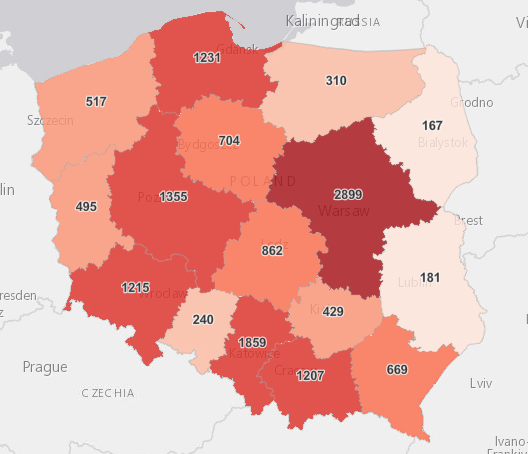
\includegraphics[width=0.8\textwidth,keepaspectratio]{img/wzgledne_bezwzgledne.png}
    \caption{Bezwzględna liczba zarażeń koronawirusem w województwach}
    \label{wzgledne_bezwzgledne}
\end{figure}

Rysunek \ref{wzgledne_bezwzgledne_fixed} prezentuje omawiane dane w nieco inny sposób. Górny wykres
przedstawia dokładnie te same wartości co \ref{wzgledne_bezwzgledne}, tylko na wykresie słupkowym -
\emph{wartość bezwzględną}.  Natomiast dolny wykres prezentuje liczbę zakażeń na 10 tys.
mieszkańców - \emph{wartość względną}. Jak widać na przykładzie wspomnianych województw
mazowieckiego i lubuskiego, poprzednie wnioski nie mają zbyt dużego sensu, kiedy uwzględni
się liczbę mieszkańców danego województwa.

\begin{figure}
    \centering
    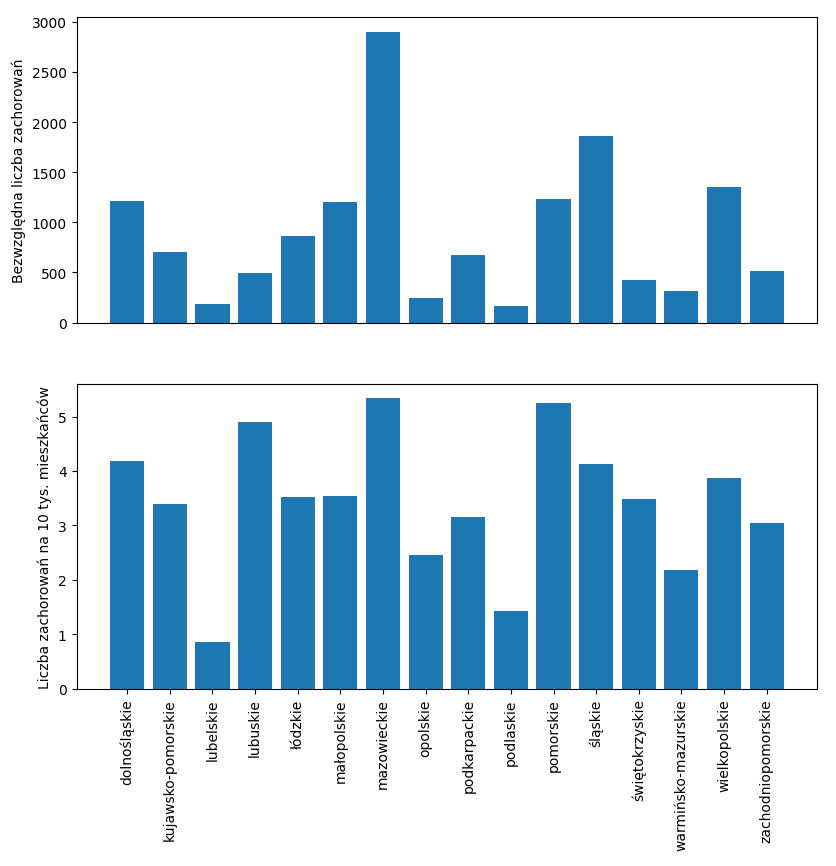
\includegraphics[width=0.8\textwidth,keepaspectratio]{img/wzgledne_bezwzgledne_fixed.png}
    \caption{Względna liczba zarażeń koronawirusem w województwach}
    \label{wzgledne_bezwzgledne_fixed}
\end{figure}

Z opisanym tutaj problemem można spotkać się dość często i w zupełnie różnych dziedzinach. Należy
więc zawsze uważać, czy mówi się o wartościach względnych czy bezwzględnych i co najważniejsze,
które z nich są faktycznie reprezentatywne dla danej dziedziny.

\section{Przykład 2: Zgony na koronawirusa w zależności do wieku}

\begin{figure}
    \centering
    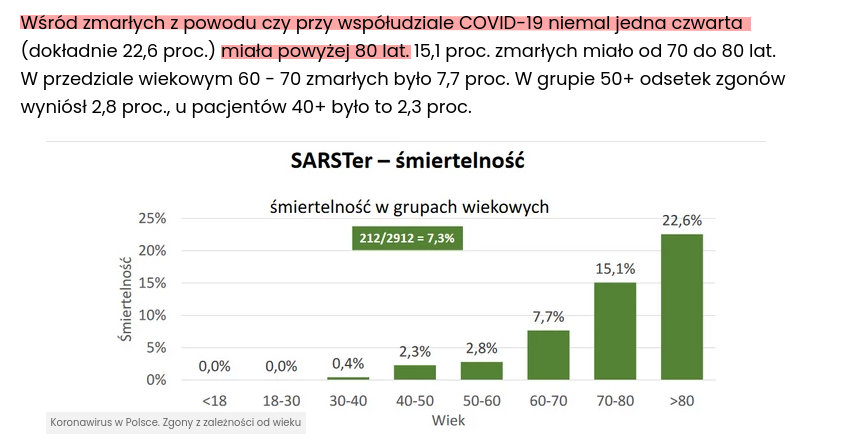
\includegraphics[width=1\textwidth,keepaspectratio]{img/wzgledne_wzgledne.png}
    \caption{Zgony na koronawirusa w zależności od wieku}
    \label{wzgledne_wzgledne}
\end{figure}

Drugi przykład jest znacznie bardziej prozaiczny, zawiera natomiast błąd trudny do wychwycenia, na
pierwszy rzut oka. Może on być popełniony przypadkowo lub z premedytacją - w tym drugim przypadku
byłaby to jednak niezwykle bezczelna manipulacja. Przedstawiony błąd został przedstawiony na rysunku
\ref{wzgledne_wzgledne} (źródło
https://www.medonet.pl/koronawirus/koronawirus-w\-polsce,koronawirus-w-polsce--smiertelnosc---co-wiemy-o-ofiarach-,artykul,07236681.html).
Na czerwono zakreślono fragment zdania, który zawiera błędną informację.  Aby pokazać, że jest ona
błędna należy zastanowić się, co przedstawia wykres. Przedstawia on śmiertelność, a więc stosunek
chorych, którzy nie przeżyli, do wszystkich chorych z danej kategorii wiekowej. Innymi słowy ze 100
chorych na covid osiemdziesięciolatków około 23 średnio umiera.  Natomiast będące częścią artykułu
zdanie zawiera zgoła inną informację: ze wszystkich zmarłych z powodu koronawirusa około 23 procent
ma powyżej 80 lat. Jak widać jest to więc zupełnie inna wartość: stosunek zmarłych z powodu
koronawirusa w wieku powyżej 80 lat do wszystkich zmarłych.  Można więc powiedzieć, że ktoś pomylił
tutaj znaczenie wartości względnych, dwie zupełnie różne proporcje. Można wysnuć z tego wniosek, że
o ile wartości bezwzględne mają znaczenie oczywiste to wartości względne można łatwo zrozumieć źle a
nawet opacznie.

\end{document}
